\chapter{Análisis del escenario legado}

A continuación se indican los roles de los participantes en el proceso de
evaluación de postulaciones. Luego se describe y discute dicho proceso.
Finalmente, se analizan las alternativas para extraer la información de las
postulaciones desde UCampus, y de esa manera poder alimentar el sistema
desarrollado en esta memoria.

\section{Participantes en el Proceso de Evaluación de Postulaciones}

% Wrappear la tabla...
\begin{table}[ht]
    \begin{center}
        \begin{tabular}{|l|l|}
            \hline \\
            Rol & Descripción \\ \hline

            Postulante & Genera una postulación a través de UCampus. Una vez
            entregada la postulación completa, éste espera por el resultado
            (aceptación o rechazo) de la misma.\\ \hline

            Miembro del Comité Académico del Programa & Evalúa las
            postulaciones, emite un voto y entrega su opinión al Coordinador de
            Magíster en forma de comentarios. Estos comentarios justifican la
            opinión del miembro correspondiente respecto a la aceptación o
            rechazo de un postulante \\ \hline

            Coordinador de Magíster / Presidente del Comité Académico & Resuelve
            una postulación. La decisión es tomada en base a las evaluaciones
            realizadas por los miembros del comité. \\ \hline

            Asistente / Funcionario del PEC & Se encarga de revisar la validez
            de los documentos adjuntados a la postulación, y deriva la
            información al Coordinador del Magíster y a los miembros del Comité
            Académico del Programa cuando corresponde. Los asistentes
            (funcionarios) son quienes llevan a cabo la mayor parte del workflow
            manual involucrado en el procesamiento de las postulaciones. \\ \hline
        \end{tabular}
    \end{center}
\end{table}


\section{Proceso a apoyar}

Tomando en cuenta el rol de cada actor, a continuación se resume el proceso que
sigue una postulación hasta lograr un veredicto de aceptación o rechazo.

% Figura
\begin{figure}[!ht]
    \begin{center}
        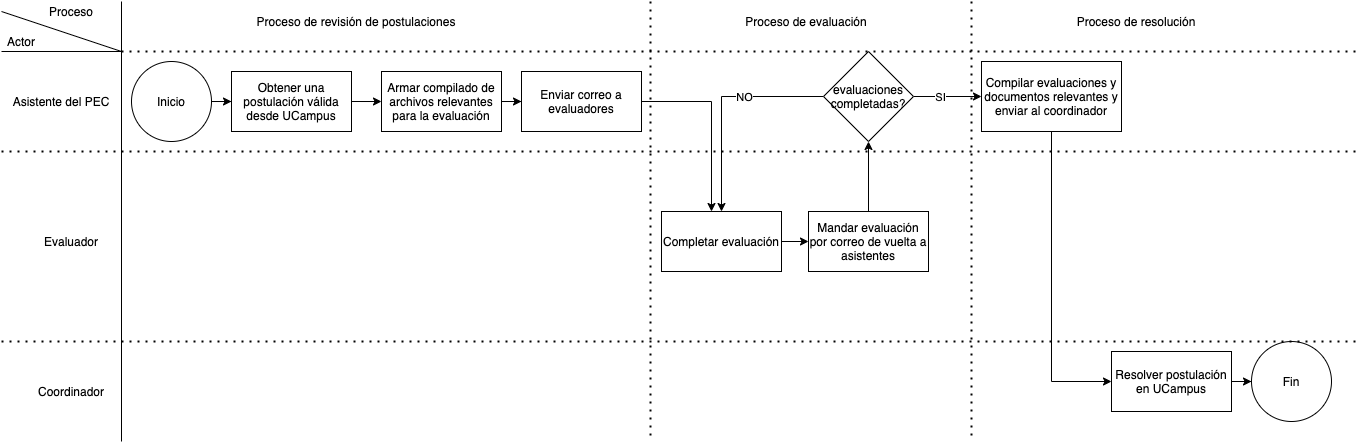
\includegraphics[scale=0.3]{imagenes/01-workflow-legado.png}
    \end{center}
    \caption{Workflow del proceso de evaluación de postulaciones}
    \label{workflow-legado}
\end{figure}

Tal como se puede ver en la figura \ref{workflow-legado}, el proceso involucra
los siguientes 7 pasos:

\begin{enumerate}
    \item Un postulante ingresa una postulación a través de UCampus.
    \item Los asistentes revisan la validez y completitud de la postulación. En
    caso de ser válida y estar completa, la información asociada a ésta se envía
    al Coordinador del Programa y a los Miembros del Comité Académico vía correo
    electrónico.
    \item El Coordinador del Programa y los Miembros del Comité Académico
    evalúan cada postulación, y emiten un juicio individual acerca de la
    aceptación o rechazo del postulante al programa, teniendo en cuenta las
    exigencias establecidas en la normativa vigente del MTI.
    \item Cada evaluador envía por correo sus evaluaciones al asistente, quien
    las recolecta y envía al Coordinador del Programa el conjunto de todas las
    evaluaciones recibidas.
    \item El Coordinador del Programa revisa todas las opiniones de los
    evaluadores y emite un veredicto acerca de la aceptación o rechazo del
    postulante.
    \item El Coordinador del Programa registra la decisión en UCampus y entrega
    a los asistentes un formulario de resolución firmado.
    \item Los asistentes envían el formulario a la Escuela de Postgrado, quien
    notifica al postulante.
\end{enumerate}

En el paso 2, la postulación puede ser devuelta al postulante para que corrija
errores en caso de que existan, o para que éste envíe los documentos faltantes.
Después de una revisión del proceso con el coordinador del programa y miembros
del comité académico, se determinó que el diseño del mismo era apropiado. Las
falencias del mismo radican principalmente en la artesanalidad e informalidad
con la que se realizan las actividades que son parte del mismo. Por lo tanto, la
automatización de algunas de esas actividades parece ser suficiente para mejorar
considerablemente la calidad y predictibilidad del proceso en términos de su
duración.

\section{Obtención de Datos desde la Plataforma UCampus}

Respecto de la obtención de datos de las postulaciones (desde UCampus), a pesar
de que exista una API publicada por su equipo desarrollador, ésta no incluye
end-points que permiten obtener los datos de las postulaciones al magíster, lo
cual va en contra del primer propósito: “permitir agilizar el proceso de
postulaciones”. 

Para resolver este problema, una solución que no involucra trabajo extra de los
usuarios es hacer scraping de la página de postulaciones de UCampus. En ella se
muestra una tabla con todas las postulaciones y un link de detalle a cada una de
ellas, desde donde se puede obtener la información de todas las postulaciones al
programa. Teniendo esta información, ya sea vía scraping o via una extensión a
la API de UCampus, es posible construir un proceso autónomo que recupere la
información de las postulaciones, sin que se requiera coordinación manual del
proceso por parte de los Asistentes o del Coordinador del Programa.

Para agilizar el procesamiento de las postulaciones, el sistema enviará avisos a
los usuarios relevantes cuando se requiere que tomen alguna acción, evitando así
que estos tengan que estar pendientes de ingresar al sistema para ver si tienen
alguna asignación sobre la cual responder. Un estudio realizado por la empresa
Microsoft constató que este envío de avisos concientiza a las personas de que
hay cosas pendientes, y aunque distrae, es preferido por su valor en la
concientización [1].

Con respecto a la facilidad de recopilación y almacenamiento de los datos
relevantes de los postulantes, usar una base de datos para dicho propósito es
mejor que mantener los datos en las cuentas de correo de los participantes en el
proceso. Si bien algunos datos están disponibles en UCampus (como los resultados
de las postulaciones, por ejemplo), las opiniones de los Miembros del Comité
Académico, entre otros datos, quedan en la cadena de correos asociada a una
publicación. Usando una base de datos, estos datos serán luego fáciles de
acceder, por ejemplo, para realizar un análisis de la efectividad y eficiencia
del procesamiento de las postulaciones.

El desarrollo de este sistema cuenta con los siguientes desafíos:

\begin{enumerate}
    \item UCampus no entrega información estructurada respecto a postulaciones
    al magíster, y se pretende que la alimentación de datos sea realizada de
    forma automática.
    \item El sistema debe automatizar el flujo de trabajo, invitando a los
    participantes (roles involucrados en el proceso) a completar sus tareas lo
    más rápido posible, manteniéndolos informados acerca de tareas que
    eventualmente ellos tengan pendientes de realizar.
    \item El sistema debe garantizar que cada actor del proceso pueda hacer sólo
    lo que su rol permite, y nada más.
\end{enumerate}


\section{Análisis de Alternativas de Interacción con UCampus}

En esta sección se describen las tareas realizadas en la búsqueda de una
solución a la extracción automática de información desde UCampus. En particular
se indican los desafíos asociados a los problemas que hay que resolver, las
alternativas para abordarlos y las propuestas de solución.

\subsection{Posible Extensión de la API de UCampus}

Una de las primeras tareas realizadas fue comunicarse con el área de desarrollo
de UCampus, para explorar la factibilidad de implementar un nuevo endpoint en su
API, con el objetivo de permitir la extracción de los datos de las postulaciones
desde una aplicación externa; en este caso, nuestro sistema de evaluación. Si
bien la respuesta fue pronta y con buena disposición, no se dió curso a la
solicitud por las siguientes razones:

\begin{itemize}
    \item El formulario de ingreso de datos y el flujo de una postulación están en
    el sistema llamado ``Workflow'', el cual está a cargo del ADI (Área de
    Infotecnologías), y por lo tanto, poco puede ayudar el Centro UCampus a la
    intervención de dicho sistema. Además, no hay una conexión directa entre el
    sistema de ADI y la plataforma UCampus, por lo que se requiere realizar bastante
    trabajo para poder contar con información de postulaciones a través de la API de
    UCampus.
    \item La respuesta desde ADI fue que los datos se encuentran encapsulados dentro
    de herramientas internas del sistema ``Workflow'', lo cual dificulta la extracción
    de datos limpios desde su base de datos.
\end{itemize}

En resumen, y aunque aún no está completamente cerrada la posibilidad de obtener
los datos desde la fuente, se hace necesario explorar otras opciones, las cuales
se detallan a continuación.

\subsection{Extracción de Datos de UCampus Usando Scrapers}

Scraping es una técnica que se usa para la extracción de datos no estructurados,
ya sea a partir de imágenes, PDFs, o páginas web, entre otros. Al no poder
obtener directamente los datos de postulaciones a través de una API (o una
interfaz de acceso a datos similar), usar un scraper es una buena alternativa
para recuperar dicha información. En este caso, los datos de las postulaciones
se encuentran accesibles a través de una interfaz Web de la plataforma UCampus,
siempre que se cuente con los derechos para ello. Este es el canal oficial tanto
para postular, como para gestionar las postulaciones.

El uso de scrapers no está exento de desafíos. Algunos de los más conocidos son
los siguientes: 

\begin{itemize}
    \item Si el sitio web que representa la fuente de datos cambia su interfaz
    de usuario, entonces se debe adaptar el scraper para extraer información del
    nuevo layout de la página.
    \item Algunos sitios web (y este es el caso de UCampus) usan Javascript en
    su interfaz (versiones modernas). Esto hace que no sea trivial la extracción
    de los datos, pues el scraper debe esperar por eventos asíncronos para poder
    extraer datos. Las librerías tradicionales de scraping [6, 7] no cuentan con
    esa capacidad.
\end{itemize}

A pesar de lo planteado anteriormente, usar un scraper es realmente la única
alternativa que existe hoy para poder extraer los datos de las postulaciones de
forma automática. Con respecto a las alternativas para hacer el scraping, se
analizaron las siguientes librerías, dado que están dentro de las más
reconocidas:

\begin{itemize}
    \item Puppeteer [3]: Librería Node.js que permite controlar una instancia de
    Chrome a través del protocolo DevTools.
    \item Selenium WebDriver [4]: Esta es una API con implementación en
    múltiples lenguajes, orientada al testing, que permite manejar un browser.
\end{itemize}

Las diferencias entre estas librerías radica principalmente en que Puppeteer
controla instancias de Chrome, mientras que Selenium es una implementación para
un navegador genérico. Ambas cumplen el propósito de extraer datos desde UCampus
sin problemas [8]. En el repositorio referenciado se muestran los resultados de
extraer ciertos datos desde UCampus con la cuenta del autor, de acuerdo a la
siguiente secuencia de pasos:

\begin{enumerate}
    \item Ingresar a UCampus con usuario y contraseña.
    \item Hacer clic en la pestaña Tareas Iniciadas.
    \item Extraer links desde una tabla. Cada caso particular (postulación)
    corresponde a una “Solicitud de Inscripción con Excepción (SIEs)”.
    \item Visitar todos los links disponibles y extraer sus datos.
\end{enumerate}

Con el objetivo de mantener la estabilidad del scraper, en el sentido de que
éste soporte la mayor cantidad de alternativas posibles para abordar los
eventuales cambios en la interfaz de usuario, puppeteer es la mejor opción. El
hecho de que la librería esté construida sobre Chromium hace que se pueda usar
todo el abanico de herramientas de Chrome para obtener datos, y manipular el
sitio web. Otro argumento para lo mismo es la frecuencia de actualizaciones. Los
drivers de Selenium mantienen su última fecha de liberación (para Python) el 1
de noviembre de 2018, mientras que Puppeteer lanzó su última versión el 26 de
febrero de 2021.

Debido a esto, y tomando en cuenta la cantidad de postulantes al MTI, resulta
válido también explorar la posibilidad de que los datos sean ingresados
manualmente al sistema por parte de sus usuarios; particularmente, por los
funcionarios del PEC.

\subsection{Carga Manual de datos de Postulaciones}

Si bien lo ideal es que los datos sean ingresados de forma automática al
sistema, no hay que perder de vista que el objetivo principal de este trabajo
es: desarrollar un sistema Web que automatice el flujo de trabajo asociado al
procesamiento de postulaciones al Magíster en Tecnologías de la Información. Con
eso en cuenta, la carga manual de datos se percibe más bien como un despropósito
en este escenario.

Por otra parte, los scrapers anteriormente descritos fueron probados con
resultados satisfactorios que, en una primera aproximación, demostraron que es
posible extraer datos no estructurados desde UCampus, y confiar en los
resultados de dicho proceso. 

\section{Formulario de Postulación al MTI}

A continuación se muestra un formulario típico de postulación al MTI,
implementado sobre la plataforma UCampus. Se han ofuscado los datos sensibles
del postulante.

\begin{figure}[!ht]
    \begin{center}
        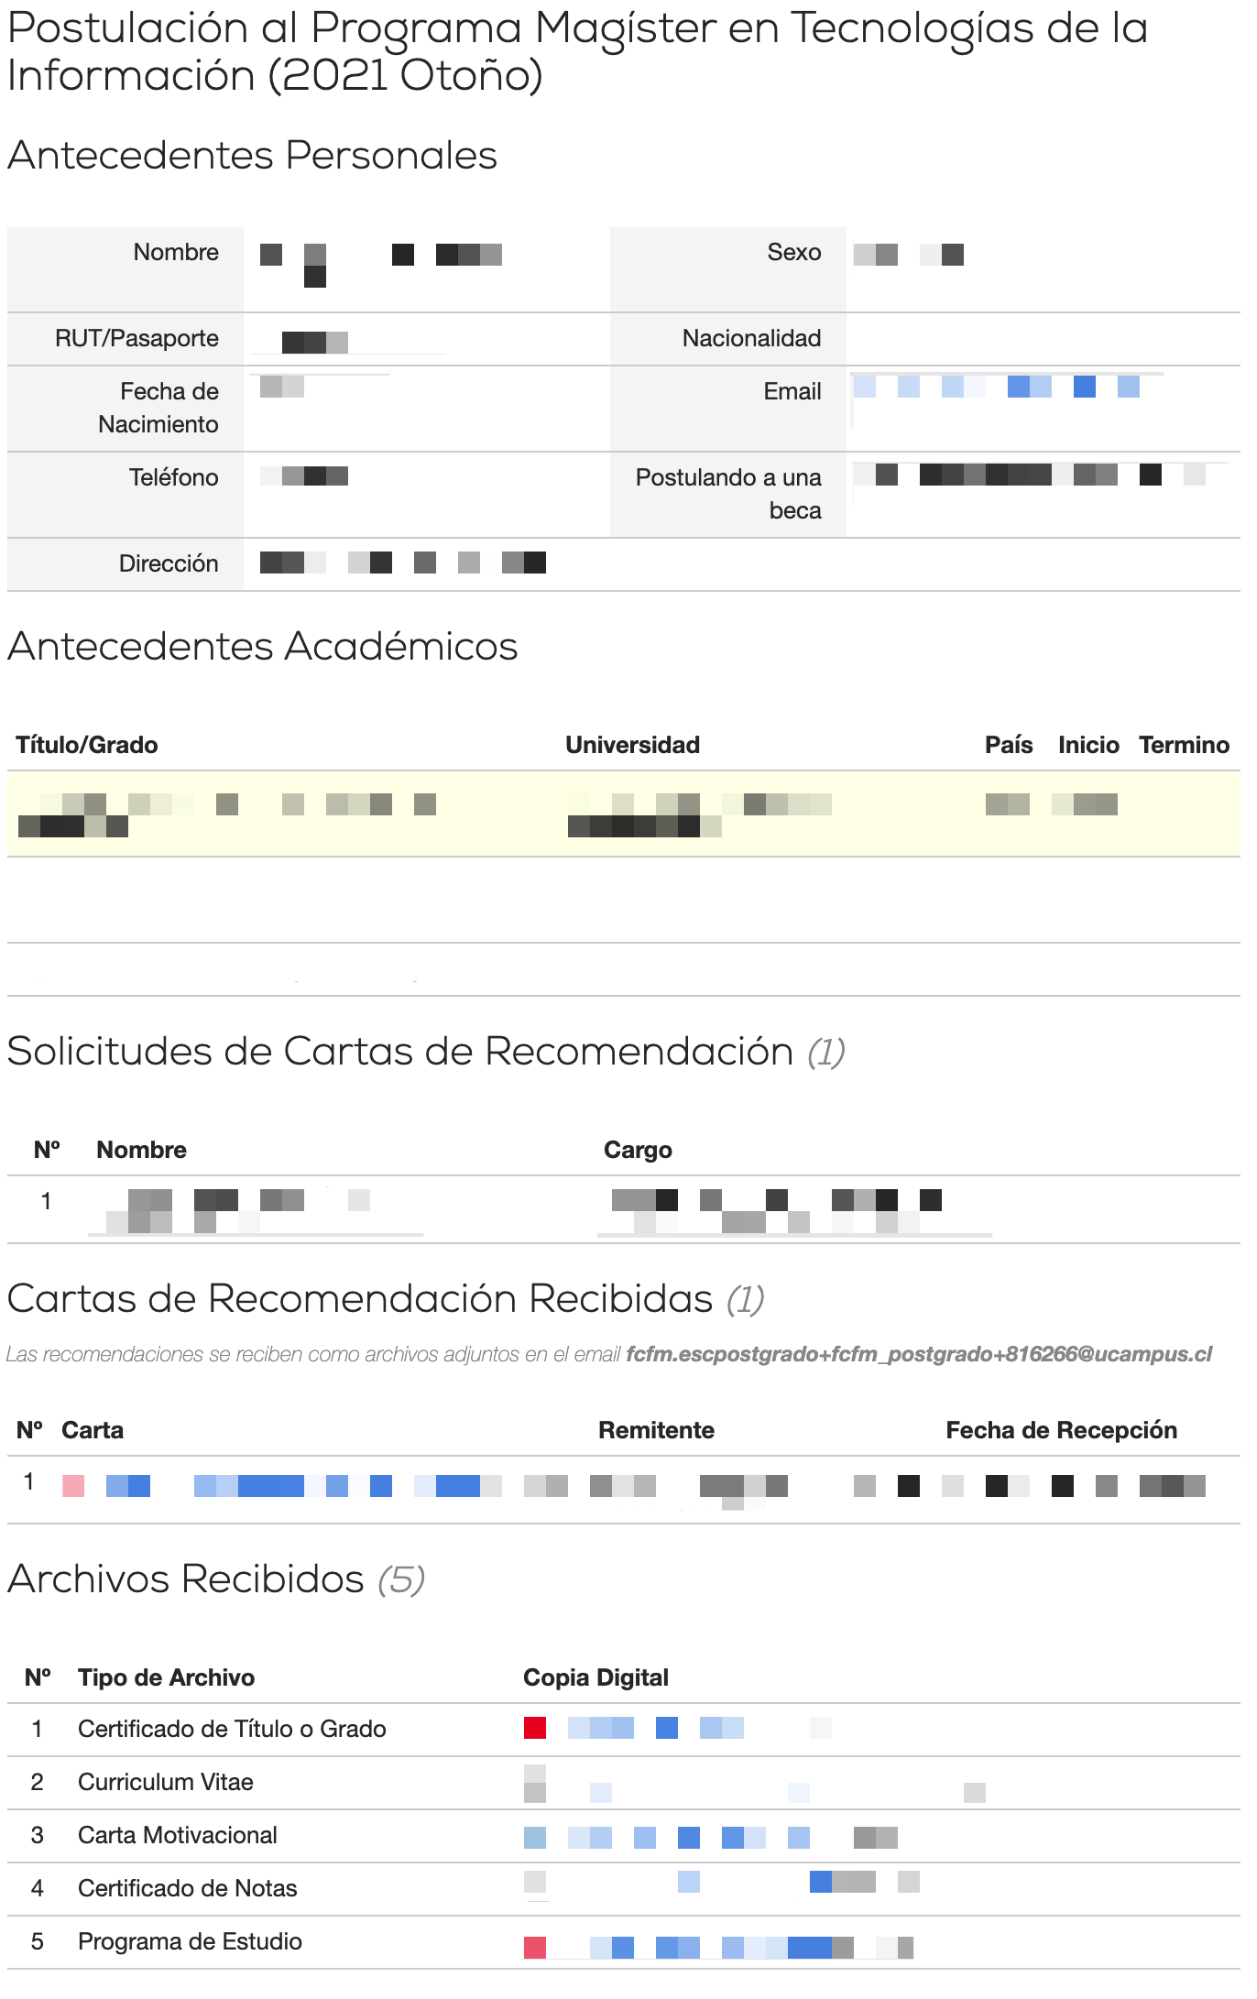
\includegraphics[scale=0.3]{imagenes/01-formulario-postulacion.png}
    \end{center}
    \caption{Formulario de postulación al Magíster en TI}
    \label{formulario-postulacion}
\end{figure}

Como se puede ver en la Figura \ref{formulario-postulacion}, una postulación
completa consta de los siguientes antecedentes:

\begin{itemize}
    \item Datos personales del alumno.
    \item Los antecedentes académicos del mismo: Título o grado, Universidad, País
    de la Universidad, Año de inicio y término de sus estudios.
    \item Solicitudes de cartas de recomendación, hechas por el postulante. Éstas se
    muestran por el nombre de cada persona a la que se le solicitó una carta de
    recomendación, su correo electrónico y su cargo.
    \item Cartas de recomendación recibidas. Éstas muestran el archivo
    correspondiente a la carta de recomendación, el nombre de la persona que lo
    envió, su email y la fecha de recepción.
    \item Los 5 archivos mandatorios de cada postulación: Certificado de título o
    grado, currículum vitae, carta motivacional, certificado de notas y el programa
    de estudio.
\end{itemize}

Algunas consideraciones a destacar del formato de los datos:

\begin{itemize}
    \item La fecha de nacimiento de un alumno sólo está presente para usuarios
    antiguos de UCampus. Usualmente ese campo sólo muestra la edad.
    \item La nacionalidad, de la misma forma, no suele estar presente en la
    postulación.
    \item La postulación puede estar a medio hacer. Vale decir, puede ser que la
    postulación no contenga las cartas de recomendación o documentos esenciales,
    y aún así el sistema permite que la misma sea enviada al coordinador del
    programa.
\end{itemize}